\chapter{Prototypes et résultats de tests préparatoires}


\section{Modèle}
\subsection{Prototype}
image ici

\subsection{Tests envisagés}
\begin{itemize}
  \item tests généraux liés à la création d'une classe (tests getters/setters) \\

\end{itemize}


\section{Réseau de neurones}
\subsection{Prototype}
\begin{figure}[H]
    \centering
    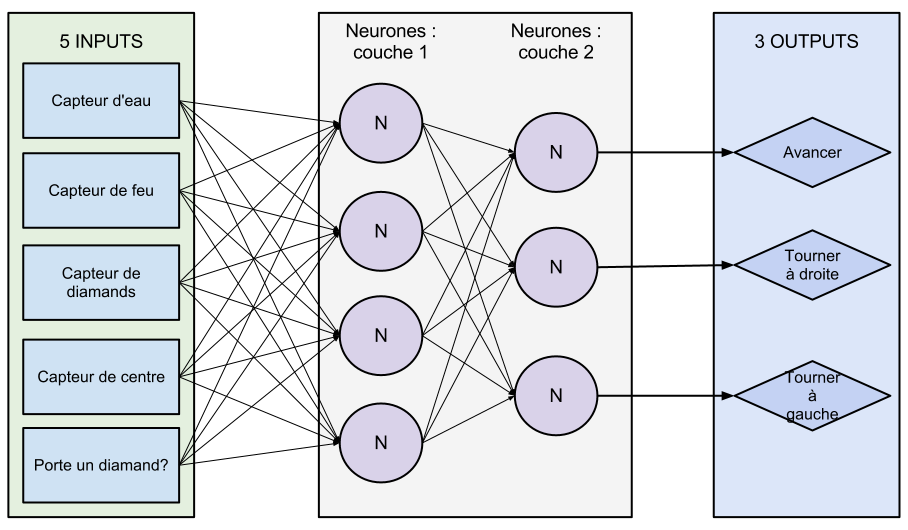
\includegraphics[width=1\textwidth]{./pictures/reseau_neurones.png}
    \caption{Réseau de neurones}
\end{figure}


\subsection{Tests envisagés}
texte ici

\section{Algorithme génétique}

\subsection{Prototype}
\begin{figure}[H]
    \centering
    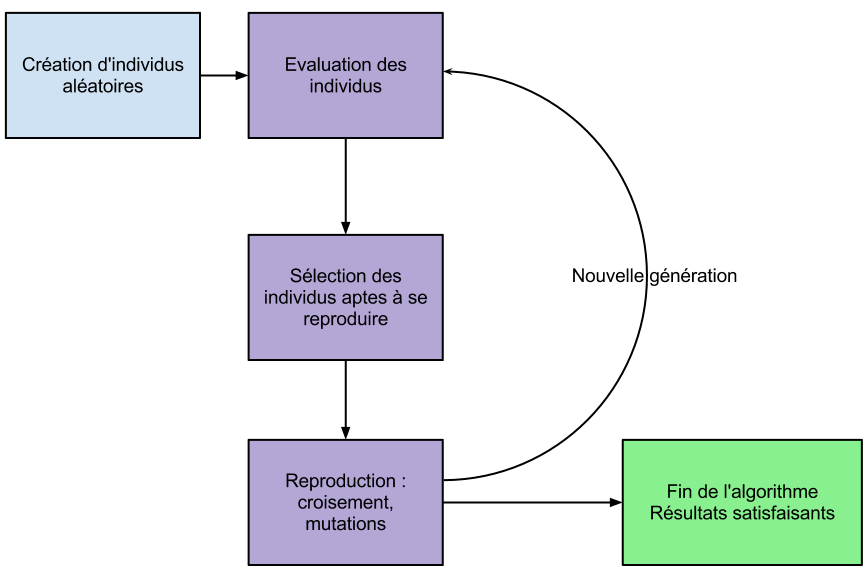
\includegraphics[width=1\textwidth]{./pictures/algo_creatures.png}
    \caption{Algo }
\end{figure}


\subsection{Tests envisagés}
texte ici

\section{Interface graphique}
\subsection{Prototype}
\begin{figure}[H]
    \centering
    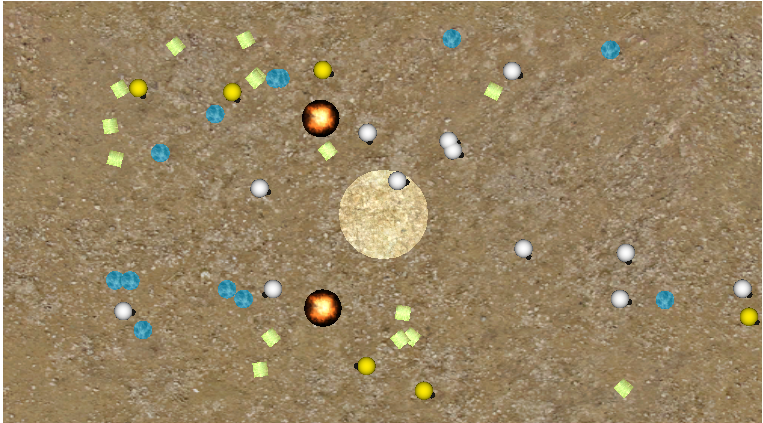
\includegraphics[width=1\textwidth]{./pictures/unity.png}
    \caption{Unity}
\end{figure}

\subsection{Tests envisagés}
Plusieurs tests à différents niveaux devront être effectués:
\begin{itemize}
  \item gestion des collisions entre les créatures et les éléments de l'environnement.\\

 \item affectation des inputs de la créature, voir si elle détecte bien les différents éléments (champs de vision)\\
 \item rendu des outputs (déplacements) de la créature
(voir le projet Unity...)
\end{itemize}
\clearpage
